\subsection{Applying the seed model to complete target expressions}
The native interface reduces each component of
Eq.~\eqref{eq:accel-expression} before combining the result. We also
applied the fast seed model directly to that complete expression,
using Kira's supplied-equation mode. This tests the form of the target
used to train the seed model and allows cancellations between its
components during the reduction.

Let $\mathcal E_{\boldsymbol b}$ be the stored IBP identities generated
from candidate seed $\boldsymbol b$, and let
$\mathcal E_{\rm bg}$ contain the stored symmetry and other background
identities. The selected equation set is
\begin{equation}
 \mathcal E(\mathcal S)=\mathcal E_{\rm bg}\cup
       \bigcup_{\boldsymbol b\in\mathcal S}\mathcal E_{\boldsymbol b}.
\end{equation}
For each requested expression, we add its defining relation
\begin{equation}
 \mathcal T_\nu-
 \sum_{\boldsymbol a\in\mathcal J_\nu}
 c_{\nu\boldsymbol a}I_{\boldsymbol a}=0.
\end{equation}
Kira eliminates the supplied system with the target expressions ordered
above their component integrals and the prescribed masters preferred
at the end of the ordering. It therefore obtains the master expansion
of $\mathcal T_\nu$ in one exact solve. The same public identity pool,
target definitions and master basis enter every compared method.

The model takes the union of candidates whose score reaches
$\tau=0.01$, using the unchanged weights and the fast inference
implementation. We tested this set both with and without an early
finite-field master check. An incomplete selected system triggers a
full-pool calculation within the remaining time allowance. The early
check compares the remaining integrals with the prescribed master
basis; exact final coefficient checks still determine whether the requested reductions
agree with their recorded answers. A global master check can require
more relations than a particular target combination needs.

These calculations begin with stored IBP identities, whose prior
generation cost is excluded for every method. The measured complete
time includes loading those inputs, prediction, equation selection and
export, Kira's exact calculation, admission checks when used, failed
attempts, fallback and final verification. Thus the result concerns
repeated reduction from a common identity pool. It does not measure
native generation of a new family's equations.


The separate development and adapter-validation collection contains 80 trials, with 74 exact completions and 6 incomplete calculations. Independent checks evaluated 2,013 target coefficients at stored finite-field points. The six adapter-validation family instances belong to the original training partition and use two batch sizes, one and sixteen targets. We retained every measured cost and selected a learned interface only when its geometric mean complete-time ratio to the full-pool control was below one and it preserved every control completion.

The validation ratio without the early master check was 1.113 across 11 complete paired batches. The full-pool control completed 0 additional batches that this learned interface did not complete. These single validation measurements select the interface and do not establish a repeatable timing gain.

The validation ratio with the early master check was 0.930 across 11 complete paired batches. The full-pool control completed 0 additional batches that this learned interface did not complete. These single validation measurements select the interface and do not establish a repeatable timing gain.

\subsection{Reserved tests of complete-expression reduction}

Validation selected the early master check. We froze this choice before applying it to the twelve original-held-out box instances used in the native comparison. The network weights and threshold remain fixed. Each instance supplies batches of one and sixteen target expressions, with five rotated repetitions per method on the same node. These are reused physical families and constructed targets; the new comparison tests the revised interface on original-held-out model data.

The controls use the full stored identity pool and a fixed set of 64 seeds ranked by their smallest index distance to any target component. The distance control uses the same exact reduction and full-pool fallback as the learned method. This first distance control proceeds directly to symbolic elimination, while the selected learned method uses the early master check. Their time ratio therefore includes both seed selection and the difference in admission checks.

The frozen plan contains 360 records. We executed 348 trials and obtained 345 exact completions; 3 measured trials failed to complete within the bounds, and 12 remaining repeats were skipped after an earlier failure. Every completed master expansion matched its exact reference, and the independent audit checked 8,460 target coefficients directly against the exported Kira reductions. Skipped repetitions have no assigned runtime.

The learned interface produced 115 exact completions, 1 failed trial and 4 skipped repeats. Completed trials used fallback 25 times.

The full-pool control produced 115 exact completions, 1 failed trial and 4 skipped repeats. Completed trials used fallback 0 times.

The distance control produced 115 exact completions, 1 failed trial and 4 skipped repeats. Completed trials used fallback 55 times.

We form a median from five successful repetitions for each method and batch, and take geometric mean ratios over complete paired batches. Descriptive 95\% intervals resample the six kinematic groups 10,000 times, preserving the relationship between profiles and batch sizes. Completion losses remain separate from these ratios.

The learned interface has a complete-time ratio of 0.944 against the full-pool control, with descriptive interval $[0.863,1.042]$ across 23 paired batches. The control completed all repeats in 0 additional batches, and the learned method completed all repeats in 0 additional batches.

The learned interface has a complete-time ratio of 0.604 against the distance control, with descriptive interval $[0.534,0.678]$ across 23 paired batches. The control completed all repeats in 0 additional batches, and the learned method completed all repeats in 0 additional batches.

The observed geometric mean complete time is 5.6\% lower than the full-pool Kira control on batches where both methods completed all five repetitions. Because the descriptive interval includes one, the aggregate timing gain across both batch sizes remains uncertain. The result applies to these constructed target expressions and their existing identity pools; it does not establish a speedup for general multiloop amplitude reductions \cite{KiraNativeAccelerationData}.

\begin{figure}[htbp]
\centering
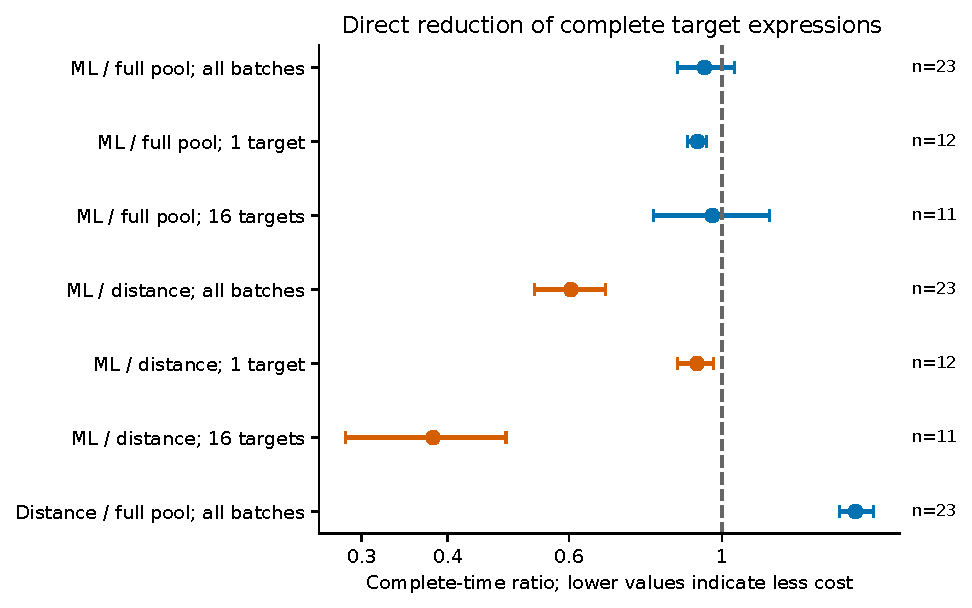
\includegraphics[width=\linewidth]{figures/whole_expression_times.pdf}
\caption{Complete-time ratios for direct reduction of complete target
expressions. Points show geometric means of five-repeat median ratios,
and intervals resample kinematic groups. The label $n$ gives the
number of complete paired batches. Failed and skipped trials remain
in the completion counts.}
\label{fig:whole-expression-time}
\end{figure}
\FloatBarrier

